\documentclass{article}

\usepackage{graphicx} % Required for inserting images
\usepackage{wrapfig}
\usepackage{amsmath} % For mathematical symbols and equations
\usepackage{natbib} % For citations   
\usepackage{floatflt}
\usepackage{amssymb}
\usepackage{booktabs}       % professional-quality tables
\usepackage{hyperref} % Web link

\newcommand\scalemath[2]{\scalebox{#1}{\mbox{\ensuremath{\displaystyle #2}}}}

\renewcommand{\arraystretch}{1.5}

\graphicspath{ {./images/} }

\title{LLaMAntino 3 8B: Further Fine-Tuning on Italian Language Using Consumer Hardware}
\author{Bruno Guzzo}
\date{Fall 2024}

\begin{document}
	
	\maketitle
	
	\begin{abstract}
		This project delves into the fine-tuning of a large language model (LLMs) for enhanced Italian language proficiency and its application in a chatbot.
		By employing 4-bit quantization, gradient checkpointing, and low-rank adaptation, we efficiently fine-tune the model on consumer hardware using well established Italian  dataset. 
		This method enables us to optimize the model's performance while minimizing computational overhead.
		To assess the impact of our fine-tuning strategy, we conduct a comprehensive evaluation using a series of Italian benchmarks, including those for question answering, commonsense reasoning, and natural language understanding.
		The project further explores the potential of incorporating a Retrieval-Augmented Generation (RAG) approach, based on a curated collection of Italian literature and novels, to enrich the chatbot's knowledge base and enhance its conversational capabilities.
	\end{abstract}
	
	\section{Introduction}
		Large Language Models (LLMs) have rapidly emerged as a transformative force in the field of artificial intelligence, demonstrating remarkable capabilities in understanding and generating human-like text. 
		These models, trained on massive datasets of text and code, leverage deep learning techniques to learn complex patterns and relationships within natural language. 
		At the core of their architecture lie several fundamental components:
		
		\begin{itemize}
			\item \textbf{Tokenization}: The process of breaking down text into smaller units, called tokens, which can be words, subwords, or even characters. This allows the model to process and represent the input text in a structured manner. 
			
			\item \textbf{Embedding}: Each token is then converted into a numerical vector, or embedding, which captures its semantic meaning in a high-dimensional space. This representation allows the model to understand relationships between words and their contextual significance.
			
			\item \textbf{Attention Mechanism}: This innovative mechanism, introduced in the seminal paper "Attention is All You Need" (Vaswani et al., 2017), enables the model to weigh the importance of different parts of the input sequence when processing information. This allows LLMs to effectively capture long-range dependencies and contextual nuances in text, a significant advancement over previous sequential models.
			
			\item \textbf{Transformers}: The dominant architecture for LLMs, transformers consist of multiple layers of self-attention and feed-forward neural networks. This structure allows for parallel processing of information, making them highly efficient and scalable for handling large datasets.
		\end{itemize}	
		
		The evolution of LLMs over the past decade has been marked by significant advancements in model size, training data, and architectural innovations. 
		Early models, such as recurrent neural networks (RNNs) and long short-term memory (LSTM) networks, faced limitations in capturing long-range dependencies and processing large amounts of data. 
		The introduction of the transformer architecture revolutionized the field, enabling the development of models with billions of parameters.
		These models have demonstrated impressive capabilities in various tasks, including text generation, translation, question answering, and code generation, sparking widespread interest and research in both academia and industry.
		
	\section{The Base Model: Meta LLaMA}
		
		\begin{figure}[h]
			\centering
			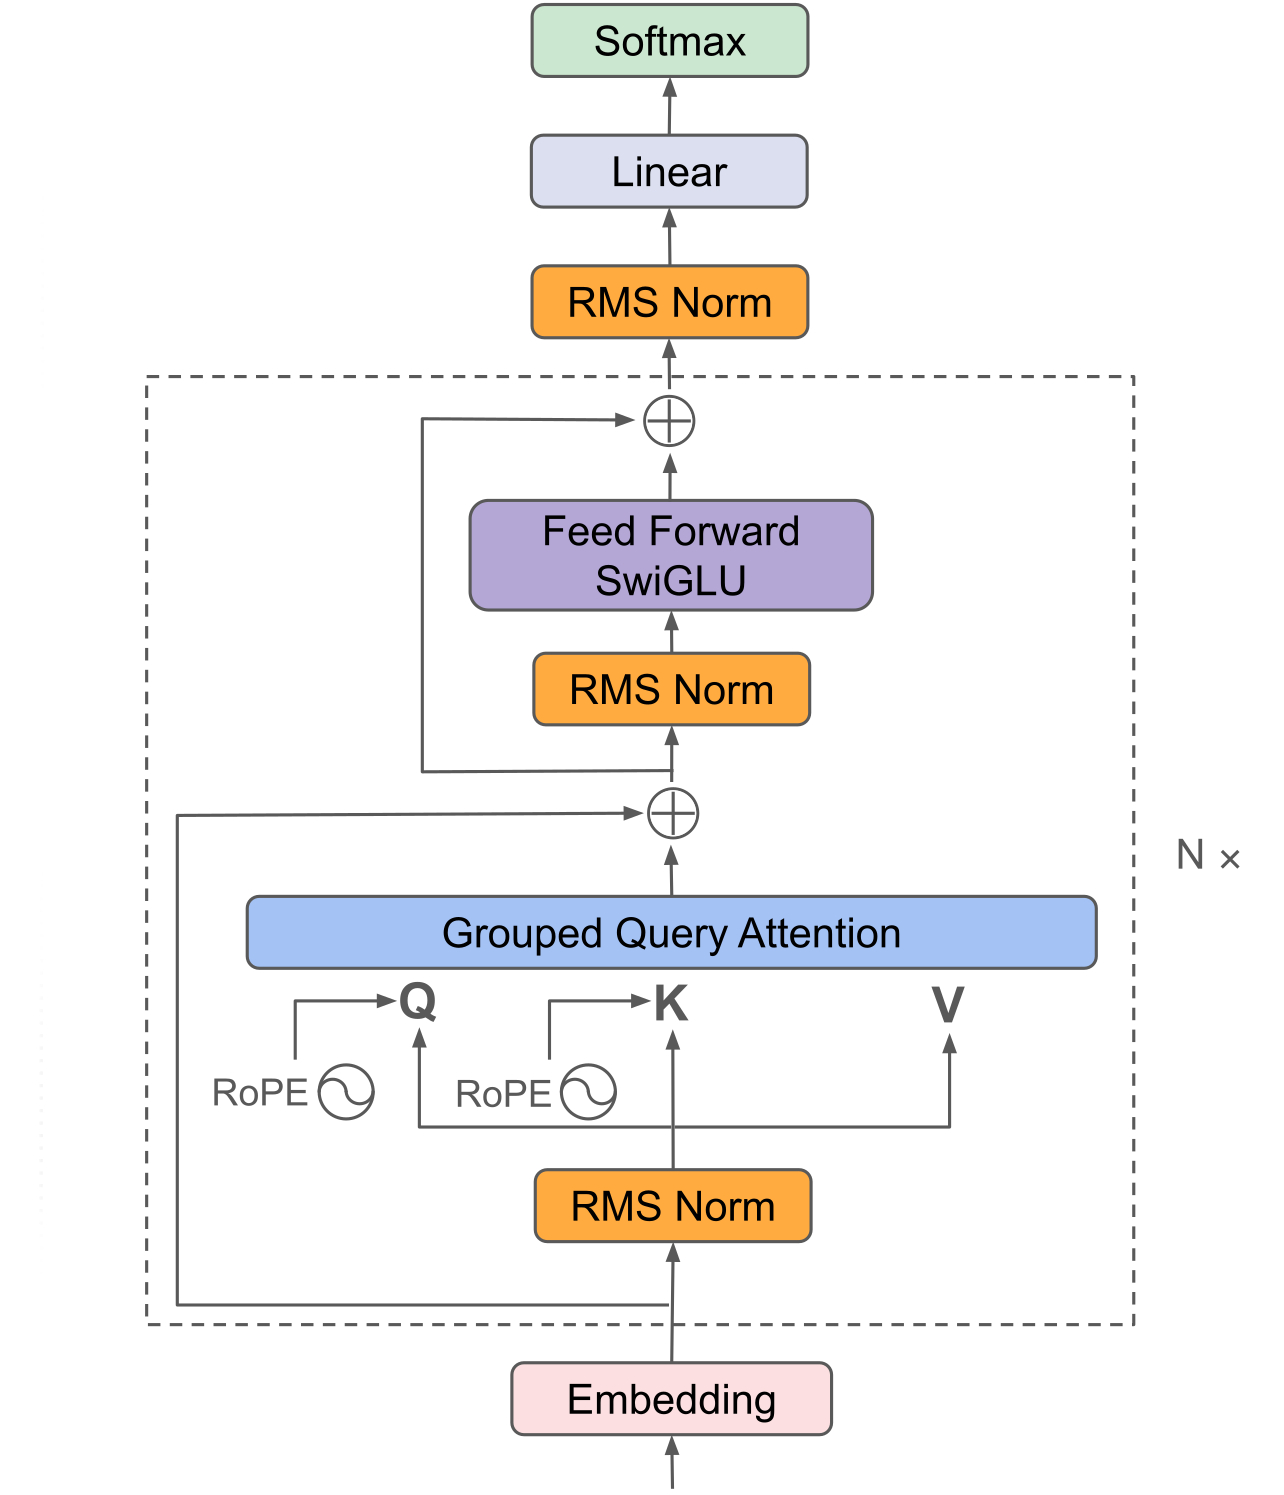
\includegraphics[width=6cm]{llama}
			\caption{LLaMa model architecture}
		\end{figure}
		
		The LLaMA model is a series of large language models (LLMs) ranging from 7B to 65B parameters, trained on trillions of tokens. 
		The goal of LLaMA is to achieve the best possible performance at various inference budgets.
		The model architecture is based on the transformer architecture, with the following modifications:
		
		\begin{itemize}
		
			\item 
				\textbf{Pre-normalization}: The input of each transformer sub-layer is normalized, rather than normalizing the output. The \textbf{RMSNorm} normalizing function is used. RMSNorm simplifies the LayerNorm (used by transfomer) by removing the re-centering operation, relying only on re-scaling. It normalizes the summed inputs to a neuron using the Root Mean Square (RMS) statistic.
				\begin{align}\label{eq_rmsnorm}
					\begin{split}
						& \bar{a}_i = \frac{a_i}{\text{RMS}(\mathbf{a})} g_i, \quad \text{where}~~ \text{RMS}(\mathbf{a}) = \sqrt{\frac{1}{n} \sum_{i=1}^{n} a_i^2}.
					\end{split}
				\end{align}
			
			\item
				\textbf{SwiGLU activation function}: The ReLU non-linearity is replaced with the SwiGLU (Swish-Gated Linear Unit) activation function. \\
				It is a combination of the \textbf{Swish activation function} and the \textbf{Gated Linear Unit} (GLU).
				
				\begin{align}\label{eq_swish_func}
					\begin{split}
						Swish(x) = x \cdot \sigma(x),  \quad GLU(x) = x \cdot \sigma(Wx + b)
					\end{split}
				\end{align}
				\begin{align}
					SwiGLU(x) = x \cdot \sigma(\beta \cdot x) + (1 - \sigma(\beta \cdot x)) \cdot (Wx + b)
				\end{align}
				
				Where \textbf{W}, \textbf{b} and $\boldsymbol{\beta}$  are trainable parameters. \\
				SwiGLU is \textbf{non-monotonic}, this allows it to capture complex non-linear relationships between input and output.
			
			\item 
				\textbf{Rotary Position Embeddings}: Absolute positional embeddings are removed, and instead rotary positional embeddings (RoPE) are used at each layer of the network to compute query and key. \textbf{RoPE} is based on the idea of using a rotation matrix to control the inner product between query and value vectors.
				Let $x_m \in \mathbb{R}^d$ and $x_n \in \mathbb{R}^d$ be two word embeddings at positions $m$ and $n$, respectively. Let $q_m$ and $k_n$ be the corresponding query and key vectors. RoPE encodes the relative position information by rotating $q_m$ and $k_n$ by an angle that is proportional to $m-n$. The rotated vectors are then used to compute the inner product. Then, \textbf{the rotation matrix} is defined as follows: 
				\begin{equation}
					\scalemath{0.75}{
						R^d_{\Theta,m} = 
						\begin{pmatrix}
							\cos{m\theta_1}& -\sin{m\theta_1}&0&0&\cdots&0&0\\
							\sin{m\theta_1}&\cos{m\theta_1}&0&0&\cdots&0&0 \\
							0&0&\cos{m\theta_2}& -\sin{m\theta_2}&\cdots&0&0\\
							0&0&\sin{m\theta_2}&\cos{m\theta_2}&\cdots&0&0 \\
							\vdots&\vdots&\vdots&\vdots&\ddots&\vdots&\vdots\\
							0&0&0&0&\cdots&\cos{m\theta_{d/2}}& -\sin{m\theta_{d/2}}\\
							0&0&0&0&\cdots&\sin{m\theta_{d/2}}&\cos{m\theta_{d/2}}
						\end{pmatrix}
					}
					\label{fn:rope-RMat}
				\end{equation}
				Where $\Theta = \{\theta_i = 10000^{-2(i-1)/d}, i \in [1, 2, ..., d/2]\}$ is a set of pre-defined parameters.
				The inner product of the rotated vectors is then computed as follows:
				\begin{equation}
					q_m^T k_n = (R_{\Theta,m}^{d} W_q x_m)^T (R_{\Theta,n}^{d} W_k x_n) = x_m^T W_q R_{\Theta,n-m}^{d} W_k x_n
					\label{q_k_inner_product}
				\end{equation}
				Where $R_{\Theta,n-m}^{d} = (R_{\Theta,m}^{d})^T R_{\Theta,n}^{d}$. \\
				This inner product decays with increasing relative distance $|m - n|$. This is due to the rotation matrix $R_{\Theta,n-m}^{d}$ becoming more diagonal and thus decreasing the overall cosine value of the angel between $q$ and $k$ vectors.
				
				
		\end{itemize}
		
		\begin{table*}[h]
			\center
			\begin{tabular}{ccccccc}
				\toprule
				params & dimension & $n$ heads & $n$ layers & learning rate & batch size & $n$ tokens \\
				\midrule
				6.7B  & 4096 & 32 & 32 & $3.0e^{-4}$ & 4M & 1.0T \\
				13.0B & 5120 & 40 & 40 & $3.0e^{-4}$ & 4M & 1.0T \\
				32.5B & 6656 & 52 & 60 & $1.5e^{-4}$ & 4M & 1.4T \\
				65.2B & 8192 & 64 & 80 & $1.5e^{-4}$ & 4M & 1.4T \\
				\bottomrule
			\end{tabular}
			\caption{\textbf{LLaMA Model sizes, architectures, and optimization hyper-parameters}}
		\end{table*}  
		
	\section{LLaMA 3}	
		LLaMA 3 is a series of large language models (LLMs) developed by Meta AI. It is the successor to the LLaMA model, featuring significant enhancements in terms of scale, performance, and capabilities. A key improvement from LLaMA to LLaMA 3 is the adoption of the \textbf{Grouped Query Attention} (GQA). It is a type of attention mechanism that groups the queries into a smaller number of groups where each group shares a single key and value. This strategy reduces the number of attention weights that need to be computed leading to faster training and computation.
		
	
		\begin{table*}[h]
			\center
			\begin{tabular}{ |p{4cm}|p{4cm}|p{4cm}| }
				\hline
				\textbf{Feature} & \textbf{LLaMA} & \textbf{LLaMA 3} \\
				\hline
				\textit{Normalization} & RMSNorm (before self-attention) & RMSNorm (before self-attention) \\
				\hline
				\textit{Activation Function} & SwiGLU & SwiGLU \\
				\hline
				\textit{Positional Embedding} & RoPE & RoPE \\
				\hline
				\textit{Attention} & Standard Multi-Head Attention & Grouped Query Attention (GQA) \\
				\hline
				\textit{Attention Mask} & No attention mask & Attention mask to prevent self-attention between different documents in the same sequence \\
				\hline
				\textit{Tokenizer} & SentencePiece Byte Pair Encoding (BPE) & SentencePiece BPE with Tiktoken vocabulary \\
				\hline
				\textit{Vocabulary Size} & 32,000 tokens & 128,000 tokens \\
				\hline
				\textit{Context Window} & 2048 tokens & 128K tokens \\
				\hline
			\end{tabular}
			\caption{\textbf{LLaMA 3 and LLaMA key differences}}
		\end{table*}  
	
		LLaMA 3 undergoes a post-training process that aligns it with human feedback. 
		This process involves \textbf{Supervised Fine-Tuning} (SFT) and \textbf{Direct Preference Optimization} (DPO). SFT is conducted on a mixture of human-annotated and synthetically-generated data, while DPO utilizes human-annotated preference data.
		
	\section{LLaMAntino 3 8B}
	\textbf{LLaMAntino 3 8B} 'ANITA' is Italian language LLM based on the Meta's LLaMA 3 8 billion parameters model. It is developed and maintained by the \textbf{SWAP Team} of the Bari University, Italy. It is fine-tuned using a combination of \textbf{Supervised Fine-Tuning} (SFT) and \textbf{Dynamic Preference Optimization} (DPO) to achieve superior performance in the Italian language. \\
	The fine-tuning process involved two main steps: 
	
	\begin{itemize}
		\item 
			\textbf{Model Supervised Fine-Tuning}: The starting point is the \textbf{meta-llama/Meta-Llama-3-8B-Instruct} model, an instruction tuned version of the base LLaMa 3 8B model. 
			Then, it has been fine-tuned using a dataset named \textbf{Chat-Error/wizard\_alpaca\_dolly\_orca}, this dataset is a combination of three well-known datasets: WizardLM\_Orca, Dolly-v2\_Orca, and Alpaca\_Orca. 
			It consists of 100K prompts organized into system, instruction, input, and output fields in English language.	The model was fine-tuned using the \textbf{Unsloth framework} on an NVIDIA H100 64GB GPU card.
		
		\item 
			\textbf{Model Direct Preferences Optimization}: After SFT, DPO was applied to align the model's outputs with human preferences. For this purpose, the \textbf{mlabonne/orpo-dpo-mix-40k} dataset has been used, which contains approximately 40k examples from various sources like \textbf{Capybara-Preferences}, \textbf{distilabel-intel-orca-dpo-pairs}, and \textbf{ultrafeedback\\-binarized-preferences-cleaned}.
			The DPO process was also conducted using Unsloth on an NVIDIA H100 64GB GPU card.
	\end{itemize}
	
	To adapt the model to the Italian language, we used the \textbf{gsarti/clean\_mc4\_it} dataset, which is a cleaned version Italian split of the multilingual colossal Common Crawl's \textbf{Web Crawl Corpus} (mC4).
	This dataset has been used with the same SFT strategy as before, formatting the prompts according to the standard LLaMA 3 template. \\
	Then, the model has been evaluated using several benchmarks, including \textbf{MMLU}, \textbf{HellaSwag},\textbf{ A12 Reasoning Challenge} (arc\_c), TruthfulQA, Winogrande, and GSM8K. 
	The results showed outstanding performance compared to similar and larger models, demonstrating the effectiveness of our fine-tuning strategy.
	
	\begin{table*}[h]
		\center
		\begin{tabular}{cc}
			\toprule
			\textbf{Metric} & \textbf{Value} \\
			\midrule
			Avg. & 0.6160 \\
			Arc\_IT & 0.5714 \\
			Hellaswag\_IT &	0.7093 \\
			MMLU\_IT & 0.5672 \\
			\bottomrule
		\end{tabular}
		\caption{\textbf{LLaMAntino 3 'ANITA' Main Benchmark Result}}
	\end{table*}  

	\section{Optimizations}
	Prior to running fine-tuning experiments on LLaMAntino 3 model various optimization strategy is needed. This strategies ensure that the model can run and train on a consumer based hardware without causing out of memory errors or being too slow. 
	The optimization strategy used is the following.
	
	\subsection{Quantization}  
	Large neural networks, are computationally expensive and memory-intensive. This makes them difficult to deploy on resource-constrained devices. Quantization addresses this by reducing the numerical precision of the network's weights and activations, typically from 32-bit floating-point to lower bit-depth representations like 8-bit or 4-bit integers. The core idea behind quantization is to map the range of real-valued weights and activations to a smaller set of quantized values. A common approach is to use an affine mapping:
	\begin{equation}
		r=S(q-Z)
	\end{equation}
	Where \textbf{r} is the real value, \textbf{q} is the quantized value, \textbf{S} is the scale factor and \textbf{Z} is the zero-point. \\
	To minimize accuracy loss, quantized training simulates the effects of quantization during the training process. This allows the network to adapt to the lower precision representation. During training, weights and activations are quantized in the forward pass, but gradients are still computed and updated in floating-point.
	
	
	\subsection{Low Rank Adaptation (LoRA)}
	The core idea of Low-Rank Adaptation (LoRA) is rooted in the observation that the changes in a model's weights during adaptation to a new task often exhibit a low rank.
	This means that the updates to the weight matrices can effectively be represented by a much smaller set of basis vectors. LoRA leverages this property to significantly reduce the number of trainable parameters during adaptation. \\
	Consider a \textbf{pre-trained weight matrix} $W \in \mathbb{R}^{d \times k}$ within a neural network layer, such as a fully connected layer or an attention head in a Transformer model. During adaptation, this weight matrix is typically updated through gradient descent, resulting in a change $\Delta W$. LoRA posits that $\Delta W$ can be approximated by a \textbf{low-rank decomposition}:
	\begin{equation}
		\Delta W \approx B A
	\end{equation}
	Where $A \in \mathbb{R}^{r \times k}$ and $B \in \mathbb{R}^{d \times r}$ are matrices with $r \ll \min(d, k)$. Here, $r$ represents the \textbf{rank of the decomposition}, which is assumed to be much smaller than the original dimensions of the weight matrix.
	The forward pass through the layer is then modified to incorporate the low-rank update:
	\begin{equation}
	h = W x + B A x = (W + B A) x
	\end{equation}
	Where $x$ is the input to the layer and $h$ is the output and $\Delta W x$ is also scaled by $\frac{\alpha}{r}$, where $\alpha$ is a constant in $r$. \\
	During training, \textbf{the original weight matrix $W$ is frozen}, and only the matrices $A$ and $B$ are updated. Both $A$ and $B$ are initialized using a random Gaussian distribution.
	By training only the low-rank matrices, the number of trainable parameters is significantly reduced, leading to \textbf{substantial memory savings}.
	
	\subsection{Gradient Checkpointing}  
	Gradient checkpointing is a technique used to reduce the memory consumption of deep neural network training. 
	It is based on the idea that instead of storing all intermediate activations of a neural network during the forward pass, only a subset of these activations need to be stored.
	The remaining activations can be recomputed during the backward pass, thereby trading off computation time for memory savings.
	Let's consider a neural network with $n$ layers. We can denote the activations of the network at layer $i$ as $a_i$. The forward pass of the network can be written as:
	\begin{equation}
		a_i = f_i(a_{i-1}, w_i)
	\end{equation}
	Where $f_i$ is the function computed by layer $i$ and $w_i$ are the weights of layer $i$.
	The backward pass of the network can be written as:
	\begin{equation}
	\frac{\partial L}{\partial a_{i-1}} = \frac{\partial L}{\partial a_i} \frac{\partial a_i}{\partial a_{i-1}}
	\end{equation}
	Where $L$ is the loss function. To compute the gradients of the loss function with respect to the activations, we need to store all the activations $a_i$ during the forward pass. This can be \textbf{memory-intensive}, especially for deep neural networks.
	Gradient checkpointing addresses this issue by only storing a subset of the activations, called checkpoints. 
	Let's denote the checkpoints as $c_k$, where $k$ is the index of the checkpoint. The forward pass of the network with gradient checkpointing can be written as:
	\begin{gather}
		a_i = f_i(a_{i-1}, w_i) \text{ if $i$ is not a checkpoint} \\
		c_k = a_i \text{ if $i$ is a checkpoint}
	\end{gather}
	During the backward pass, the activations that are not checkpoints are recomputed from the nearest checkpoint ($a_i = f_i(a_{i-1}, w_i)$). The backward pass with gradient checkpointing can be written as:
	\begin{gather}
		\frac{\partial L}{\partial a_{i-1}} = \frac{\partial L}{\partial a_i} \frac{\partial a_i}{\partial a_{i-1}} \text{ if $i$ is not a checkpoint} \\
		\frac{\partial L}{\partial c_k} = \frac{\partial L}{\partial a_i} \frac{\partial a_i}{\partial c_k} \text{ if $i$ is a checkpoint}
	\end{gather}
	
	\section{LLaMAntino 3 8B Further Fine-Tuning}
	The objective of this project is to test wether is possible to extend further the capabilities of LLaMAntino 3 model to generalize and handle Italian language tasks, such as chatting.
	Since the adoption of already discussed optimization strategy has proved to be needed run this kind of model locally, we run some of the same benchmark proposed by the authors to check how these optimizations impact the overall model permanence.   
	To save time, we choose to adopt a subset 0.20\% of the proposed datasets used by the benchmarks chosen by the authors.  
	\begin{table*}[h]
		\center
		\begin{tabular}{ccc}
			\toprule
			\textbf{Metric} & \textbf{Original Value} & \textbf{Optimized Value} \\
			\midrule
			Avg. & 0.6160 & xyz \\
			Arc\_IT & 0.5714 & xyz \\
			Hellaswag\_IT &	0.7093 & xyz \\
			\bottomrule
		\end{tabular}
		\caption{\textbf{LLaMAntino 3, 4-bit Quantization, 20\% Dataset}}
	\end{table*}
	The first way we choose to try extend the model generalization capability and enhance its knowledge regarding the Italian language it to fine tune the model to whole Italian Wikipedia dataset, available online. 
	This first idea has been justified since part of this dataset - and its variants - has been commonly used in the training of successful LLMs like the Open AI's GPT family. The dataset we choose has roughly 1.83M rows with field such as title, text and url, more details can be found \href{https://huggingface.co/datasets/wikimedia/wikipedia/viewer/20231101.it}{here} . 
	   
	
	
	
		
	\section{Related Work}
	Review existing research and literature relevant to your topic.
	
	\section{Methodology}
	Describe the methods you used to conduct your research.
	
	\section{Results}
	Present your findings and data. Use tables and figures to illustrate your results.
	
	\section{Discussion}
	Interpret your results and discuss their implications. Relate your findings to existing research.
	
	\section{Conclusion}
	Summarize your main findings and conclusions. Discuss limitations and future work.
	
	\bibliographystyle{plainnat}
	\bibliography{references} % Replace "references" with the name of your .bib file
	
\end{document}